%-----------------------------------------------------------------------------%
%                                                                             %
%    Anh�nge					                                             					  %
%                                                                             %
%-----------------------------------------------------------------------------%

\appendix
\chapter{Appendix}

\section{CoP Cost Implementation for Contact Dynamics}\label{app:ContactCoP}
This section contains the implementation of the \gls{CoP} cost for contact dynamics action models, integrated into the open-source framework Crocoddyl within the context of this thesis. 

For space-saving reasons, only the two core files are presented, each with shortened comments. The complete versions of these files, associated Python bindings, related files and a functional unit test can be traced in the associated pull request (\href{https://github.com/loco-3d/crocoddyl/pull/792}{\#792}).

\subsection{contact-cop-position.hpp}
\lstinputlisting{./code/contact-cop-position.hpp}
\subsection{contact-cop-position.hxx}
\lstinputlisting{./code/contact-cop-position.hxx}

\section{CoP Cost Implementation for Impulse Dynamics}\label{app:ImpulseCoP}
This section contains the implementation of the \gls{CoP} cost for impulse dynamics action models, integrated into the open-source framework Crocoddyl within the context of this thesis. 

For space-saving reasons, only the two core files are presented, each with shortened comments. The complete versions of these files, associated Python bindings, related files and a functional unit test can be traced in the associated pull request (\href{https://github.com/loco-3d/crocoddyl/pull/830}{\#830}).  

\subsection{impulse-cop-position.hpp}
\lstinputlisting{./code/impulse-cop-position.hpp}
\subsection{impulse-cop-position.hxx}
\lstinputlisting{./code/impulse-cop-position.hxx}

\section{Consistency Between the Frameworks}\label{app:Consistency}
This section contains a verification of the notability consistency between the novel frameworks HyRoDyn and Pinocchio, both of which are used for computing of the robot dynamics. To this end, both the \gls{IK} and \gls{ID} of the robot are recomputed with HyRoDyn and compared with the original reference trajectories  and torques, respectively, of the \gls{OC} solution obtained by Crocoddyl.
 
\subsection{Inverse Kinematics}
\cref{fig:frameworkConsistency_ik} shows the comparison of the \gls{IK} solution obtained from \gls{OC} with the recomputation from HyRoDyn. As becomes evident, both trajectories match, which indicates that the kinematics notation between both frameworks is consistent. 
\begin{figure}[h!]
\centering	
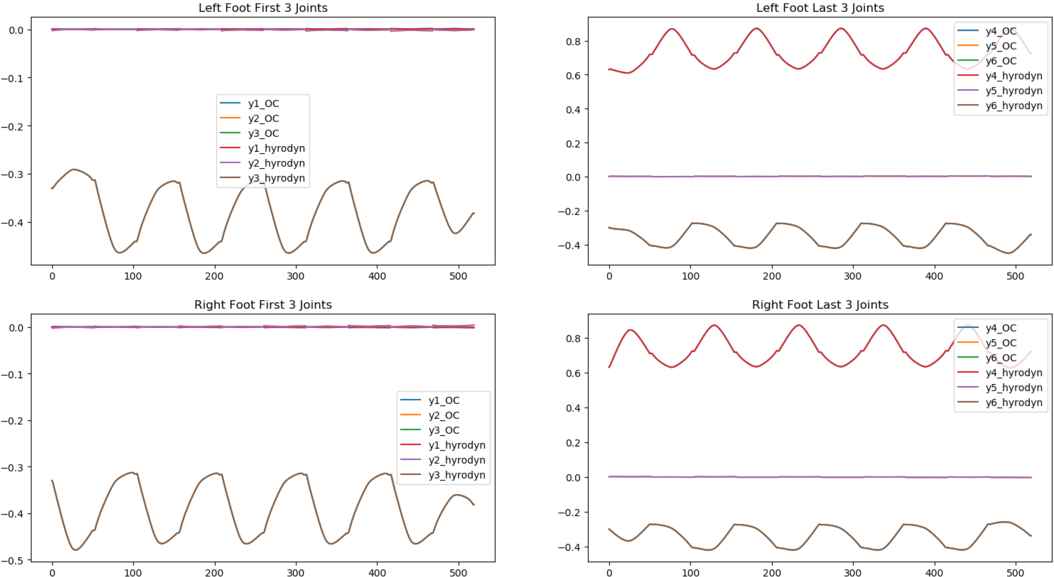
\includegraphics[width=1\textwidth]{fig/hyrodyn/ik_comparison}
\caption[\gls{IK} consistency check between HyRoDyn and Pinocchio]{\gls{IK} consistency check between the HyRoDyn and Pinocchio frameworks.}
\label{fig:frameworkConsistency_ik}
\end{figure}

\subsection{Inverse Dynamics}
\cref{fig:frameworkConsistency_id} shows the comparison of the \gls{ID} solution for optimal torque inputs from Crocoddyl with the according recomputation from HyRoDyn. As becomes evident, the torque inputs match, which proofs that also the dynamics notation between both novel frameworks is consistent.
\begin{figure}[h!]
\centering	
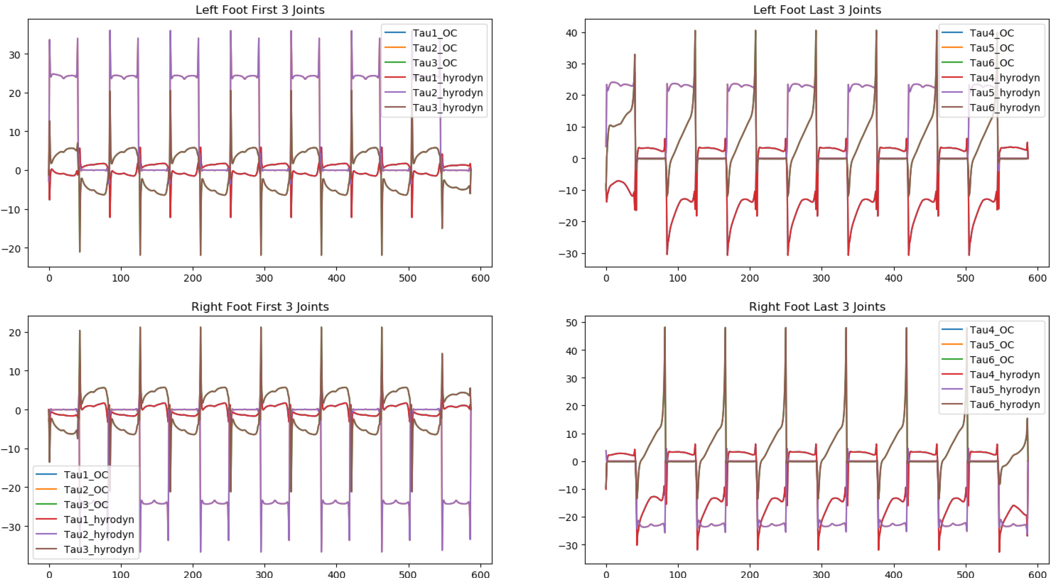
\includegraphics[width=1\textwidth]{fig/hyrodyn/id_comparison}
\caption[\gls{ID} consistency check between HyRoDyn and Pinocchio]{\gls{ID} consistency check between the HyRoDyn and Pinocchio frameworks.}
\label{fig:frameworkConsistency_id}
\end{figure}















